\testsection{Library: Groupplots}
\usepgfplotslibrary{groupplots}

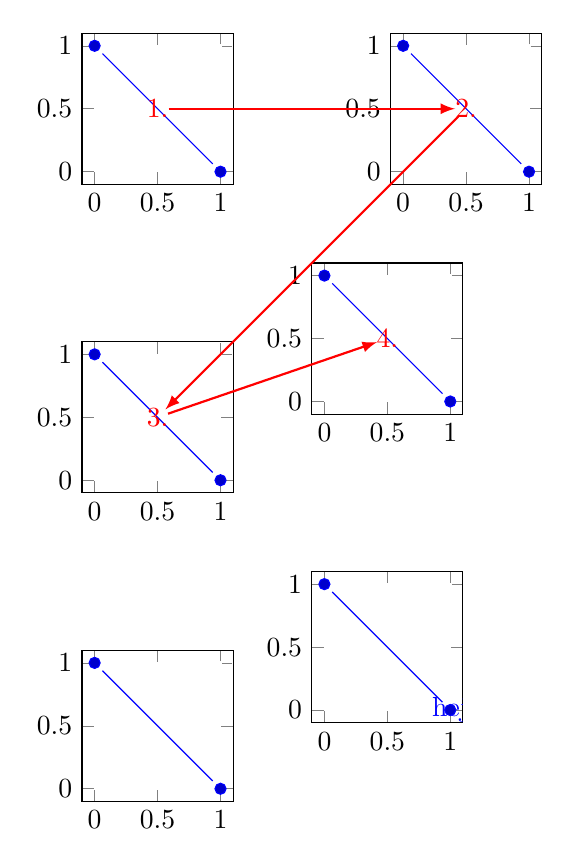
\begin{tikzpicture}[shorten >=4pt,shorten <=4pt]
  \begin{groupplot}[group style={group size=2 by 3,vertical sep=2cm},group/horizontal sep=2cm,
    height=3.5cm,width=3.5cm]
    \nextgroupplot%1
    \addplot coordinates {(0,1) (1,0)};
    \nextgroupplot
    \addplot coordinates {(0,1) (1,0)};
    \nextgroupplot
    \addplot coordinates {(0,1) (1,0)};
    \nextgroupplot[xshift=-1cm,group/vertical sep=1cm]
    \addplot coordinates {(0,1) (1,0)};
    \nextgroupplot
    \addplot coordinates {(0,1) (1,0)};
    \nextgroupplot
    \addplot coordinates {(0,1) (1,0)} node {hej};
  \end{groupplot}
  \draw[thick,>=latex,->,red] 
    (group c1r1.center) node {1.}  -- 
    (group c2r1.center) node {2.};
  \draw[thick,>=latex,->,red] 
    (group c2r1.center)  -- 
    (group c1r2.center) node {3.};
  \draw[thick,>=latex,->,red] 
    (group c1r2.center)  -- 
    (group c2r2.center) node {4.};
\end{tikzpicture}

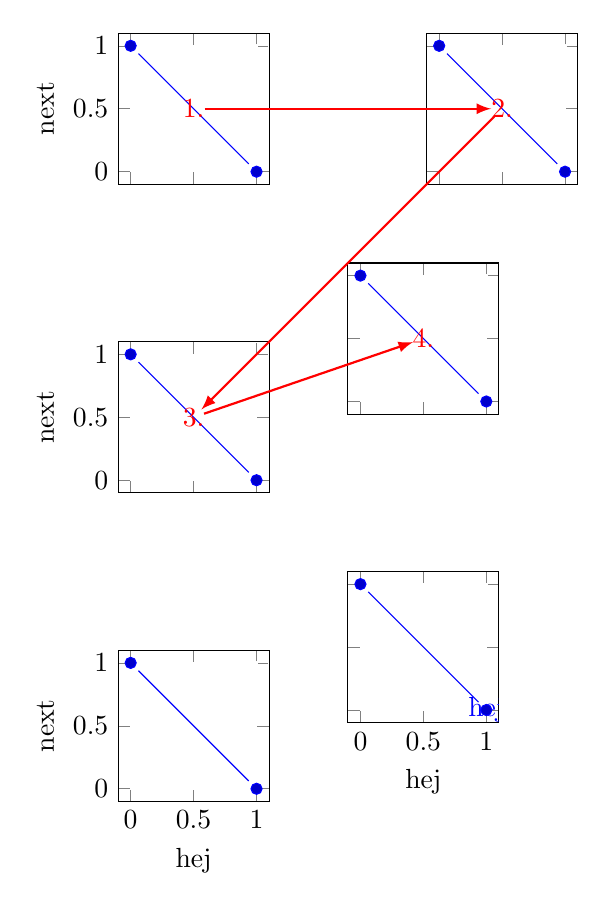
\begin{tikzpicture}[shorten >=4pt,shorten <=4pt]
  \begin{groupplot}[group style={group size=2 by 3,vertical sep=2cm,y descriptions at=edge left,x descriptions at=edge bottom},group/horizontal sep=2cm,
    height=3.5cm,width=3.5cm,xlabel={hej},ylabel={next}]
    \nextgroupplot%1
    \addplot coordinates {(0,1) (1,0)};
    \nextgroupplot
    \addplot coordinates {(0,1) (1,0)};
    \nextgroupplot
    \addplot coordinates {(0,1) (1,0)};
    \nextgroupplot[xshift=-1cm,group/vertical sep=1cm]
    \addplot coordinates {(0,1) (1,0)};
    \nextgroupplot
    \addplot coordinates {(0,1) (1,0)};
    \nextgroupplot
    \addplot coordinates {(0,1) (1,0)} node {hej};
  \end{groupplot}
  \draw[thick,>=latex,->,red] 
    (group c1r1.center) node {1.}  -- 
    (group c2r1.center) node {2.};
  \draw[thick,>=latex,->,red] 
    (group c2r1.center)  -- 
    (group c1r2.center) node {3.};
  \draw[thick,>=latex,->,red] 
    (group c1r2.center)  -- 
    (group c2r2.center) node {4.};
\end{tikzpicture}

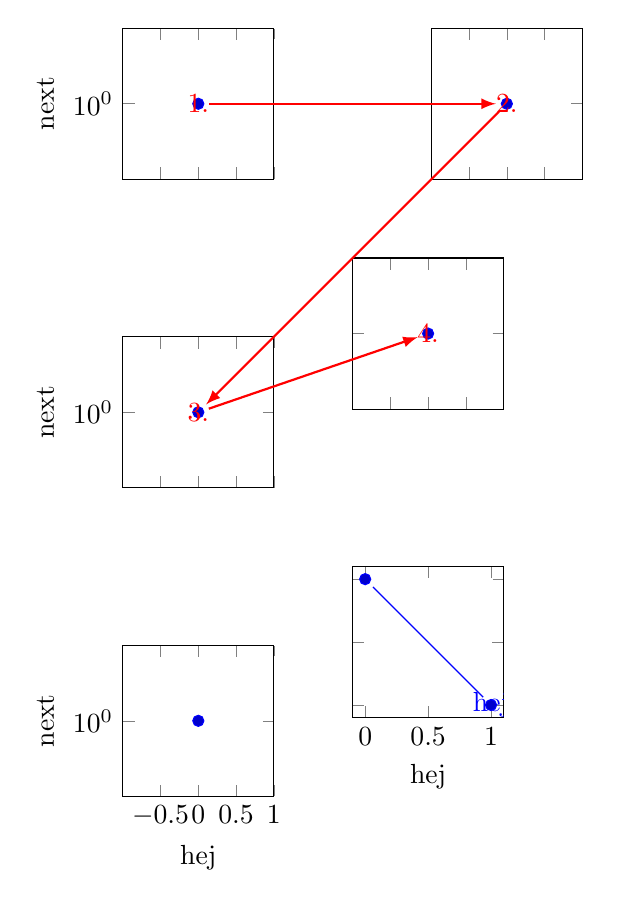
\begin{tikzpicture}[shorten >=4pt,shorten <=4pt]
  \begin{groupplot}[group style={group size=2 by 3,vertical sep=2cm,y descriptions at=edge left,x descriptions at=edge bottom},group/horizontal sep=2cm,
    height=3.5cm,width=3.5cm,xlabel={hej},ylabel={next},ymode=log]
    \nextgroupplot%1
    \addplot coordinates {(0,1) (1,0)};
    \nextgroupplot
    \addplot coordinates {(0,1) (1,0)};
    \nextgroupplot
    \addplot coordinates {(0,1) (1,0)};
    \nextgroupplot[xshift=-1cm,group/vertical sep=1cm]
    \addplot coordinates {(0,1) (1,0)};
    \nextgroupplot
    \addplot coordinates {(0,1) (1,0)};
    \nextgroupplot[ymode=linear]
    \addplot coordinates {(0,1) (1,0)} node {hej};
  \end{groupplot}
  \draw[thick,>=latex,->,red] 
    (group c1r1.center) node {1.}  -- 
    (group c2r1.center) node {2.};
  \draw[thick,>=latex,->,red] 
    (group c2r1.center)  -- 
    (group c1r2.center) node {3.};
  \draw[thick,>=latex,->,red] 
    (group c1r2.center)  -- 
    (group c2r2.center) node {4.};
\end{tikzpicture}

%%% Local Variables: 
%%% mode: latex
%%% TeX-master: "pgfplotstest"
%%% End: 
